\scanpage{9}

Considérons maintenant l'immersion projective
\diagram{\begin{tikzcd}C\arrow[r]&P(\mathcal E_3)\end{tikzcd}}
définie par $L^{\otimes3}$ en vertu de prop. 1. Alors, $C$ devient un diviseur positif sur $P(\mathcal E_3)$ simple sur $S$, \inserted{de degré relatif $3$,} il est donc défini par une \deleted{diviseur} \inserted{section sur $S$} de l'espace des $3$-formes
\[
\Phi_3(P(\mathcal E_3))\simeq P(\operatorname{Symm}_3(\mathcal E_3^\vee)).
\]
\deleted{De plus, comme}

\deleted{\uline{Supposons} que l'on se soit donné une rigidification}

Considérons la section $s$ de $P(\mathcal E_3)$ et la \deleted{``droite \unsure{des points de} \unsure{l'infini}''} \inserted{droite section $D$} de $P(\mathcal E_3)$ définis comme $P(\mathcal E_3/\mathcal E_2)$ et $P(\mathcal E_3/\mathcal E_1)$, alors on constate que $s$ est une section de $C$, et que $D$ est une ``tangente d'inflexion'' $\cdots$ par l'immersion.
\figure{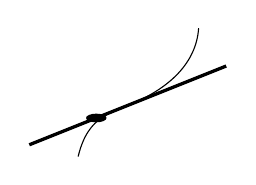
\begin{tikzpicture}[x=1cm,y=1cm]
\draw[line width=1.2pt] (0,0)--(2.5,1.0);
\draw (0.62,-0.15) .. controls (0.75,0.40) and (1.08,0.40) .. (1.25,0.50) .. controls (1.78,0.71) and (2.12,1.04) .. (2.15,1.48);
\fill (0.85,0.34) ellipse (0.13 and 0.055);
\end{tikzpicture}}

Considérons une \deleted{trivialisation} \inserted{base de $\mathcal E_3$ compatible avec} du drapeau \diagram{\begin{tikzcd}[column sep=small]0\arrow[rr,bend right=25]&\subset&\mathcal E_1\arrow[rr,bend right=25,dash]&\subset&\mathcal E_2\arrow[rr,bend right=25,dash]&\subset&\mathcal E_3\end{tikzcd}} de $\mathcal E_3$ \inserted{et commençant par $1_S\in\Gamma(S,\underline O_S)$;} [elle ``dépend de $(3+3-1)$ \inserted{$=5$} paramètres''], \deleted{par des coordonnées $z,y,x$} \inserted{i.e. une base $1,y,x$}

\margin{\diagram{$\left(\begin{array}{ccc}1&\alpha&\beta\\\diagdown&\mu&\sigma\\&\diagdown&\nu\end{array}\right)$}}

\deleted{Alors la forme $\varphi$ (définie à \unsure{unité} \deleted{\unsure{homothétie}} \inserted{multiplication près par \unsure{u}}) prend la forme [où on remplace $z$ par $1$]
\[
ax^{\unsure{2|3}}+by^3+cxy+dy^2+ex+fy+g=0
\]
\margin{$x^3\quad y^2$}
\inserted{où $y$ définit un \unsure{suppl.} de $\mathcal E_1$ dans $\mathcal E_2$ et $x$ de $\mathcal E_2$ dans $\mathcal E_3$}}

\mspage{8}
